\section{Desarrollo}
\subsection{Materiales}
Para la implementación de este sistema de medición de distancia, se requieren los siguientes materiales:

\begin{itemize}
	\item Raspberry Pi 4 (o versión compatible)
	\item Sensor ultrasónico HC-SR04
	\item Protoboard
	\item Resistencias de 1 k\textohm{} y 2 k\textohm{} (para el divisor de voltaje)
	\item Cables de conexión (jumper)
	\item Fuente de alimentación para la Raspberry Pi (5V, 3A)
\end{itemize}

\subsection{Principio de funcionamiento}
El sensor HC-SR04 mide la distancia mediante la emisión de un pulso ultrasónico de 40 kHz a través de su pin \textit{Trig}. Este pulso viaja hasta un objeto y se refleja de vuelta al sensor, donde es recibido en el pin \textit{Echo}. La Raspberry Pi mide el tiempo transcurrido entre la emisión y recepción del pulso y, utilizando la velocidad del sonido en el aire (343 m/s), calcula la distancia con la siguiente ecuación:

\begin{equation}
	\mathrm{Distancia} = \frac{\mathrm{Tiempo\ de\ respuesta} \times 34300}{2}
\end{equation}

\subsection{Conexiones eléctricas}
Para conectar el sensor HC-SR04 a la Raspberry Pi, se utiliza el siguiente esquema:

\begin{itemize}
	\item \textbf{VCC} (HC-SR04) $\rightarrow$ \textbf{5V} (Raspberry Pi)
	\item \textbf{GND} (HC-SR04) $\rightarrow$ \textbf{GND} (Raspberry Pi)
	\item \textbf{Trig} (HC-SR04) $\rightarrow$ \textbf{GPIO 23} (Raspberry Pi)
	\item \textbf{Echo} (HC-SR04) $\rightarrow$ \textbf{Divisor de voltaje} $\rightarrow$ \textbf{GPIO 24} (Raspberry Pi)
\end{itemize}

\subsubsection{Divisor de voltaje}
Dado que el pin \textit{Echo} del HC-SR04 devuelve una señal de 5V y la Raspberry Pi solo soporta señales de 3.3V en sus pines GPIO, es necesario utilizar un divisor de voltaje con resistencias:

\begin{itemize}
	\item Conectar una resistencia de \textbf{1 k\textohm{}} entre el pin \textit{Echo} y el GPIO 24 de la Raspberry Pi.
	\item Conectar una resistencia de \textbf{2 k\textohm{}} entre el GPIO 24 y GND.
\end{itemize}

Este divisor reduce la señal de 5V a aproximadamente 3.3V, protegiendo la Raspberry Pi.

\subsection{Implementación en Python}
Para obtener la medición de distancia, se utiliza un script en Python que controla la activación del sensor y mide el tiempo de respuesta. A continuación, se presenta el código para la medición de distancia:

\begin{verbatim}
	import RPi.GPIO as GPIO
	import time
	
	# Definir pines
	TRIG = 23
	ECHO = 24
	
	# Configuración de pines
	GPIO.setmode(GPIO.BCM)
	GPIO.setup(TRIG, GPIO.OUT)
	GPIO.setup(ECHO, GPIO.IN)
	
	def medir_distancia():
	GPIO.output(TRIG, True)
	time.sleep(0.00001)
	GPIO.output(TRIG, False)
	
	while GPIO.input(ECHO) == 0:
	inicio = time.time()
	
	while GPIO.input(ECHO) == 1:
	fin = time.time()
	
	duracion = fin - inicio
	distancia = (duracion * 34300) / 2  # Velocidad del sonido: 343 m/s
	
	return distancia
	
	try:
	while True:
	distancia = medir_distancia()
	print(f"Distancia: {distancia:.2f} cm")
	time.sleep(1)
	except KeyboardInterrupt:
	GPIO.cleanup()
\end{verbatim}

\subsection{Ejecución del código}
Para ejecutar el código, se debe guardar el script como \texttt{ultrasonico.py} y ejecutarlo en la Raspberry Pi con el siguiente comando:

\begin{verbatim}
	python3 ultrasonico.py
\end{verbatim}

El programa imprimirá la distancia medida en centímetros cada segundo en la terminal.

\subsection{Aplicaciones y beneficios}
La integración del sensor HC-SR04 con la Raspberry Pi permite diversas aplicaciones, entre ellas:

\begin{itemize}
	\item Detección de obstáculos en robótica
	\item Medición de niveles en depósitos de líquidos
	\item Sistemas de asistencia para estacionamiento
	\item Sensores de proximidad en automatización industrial
\end{itemize}

Este proyecto permite comprender la medición ultrasónica y su aplicación en proyectos de control y automatización, reforzando la manipulación de hardware con Raspberry Pi.

\subsection{Fotografías de la Actividad}

\begin{figure}[h]
	\centering
	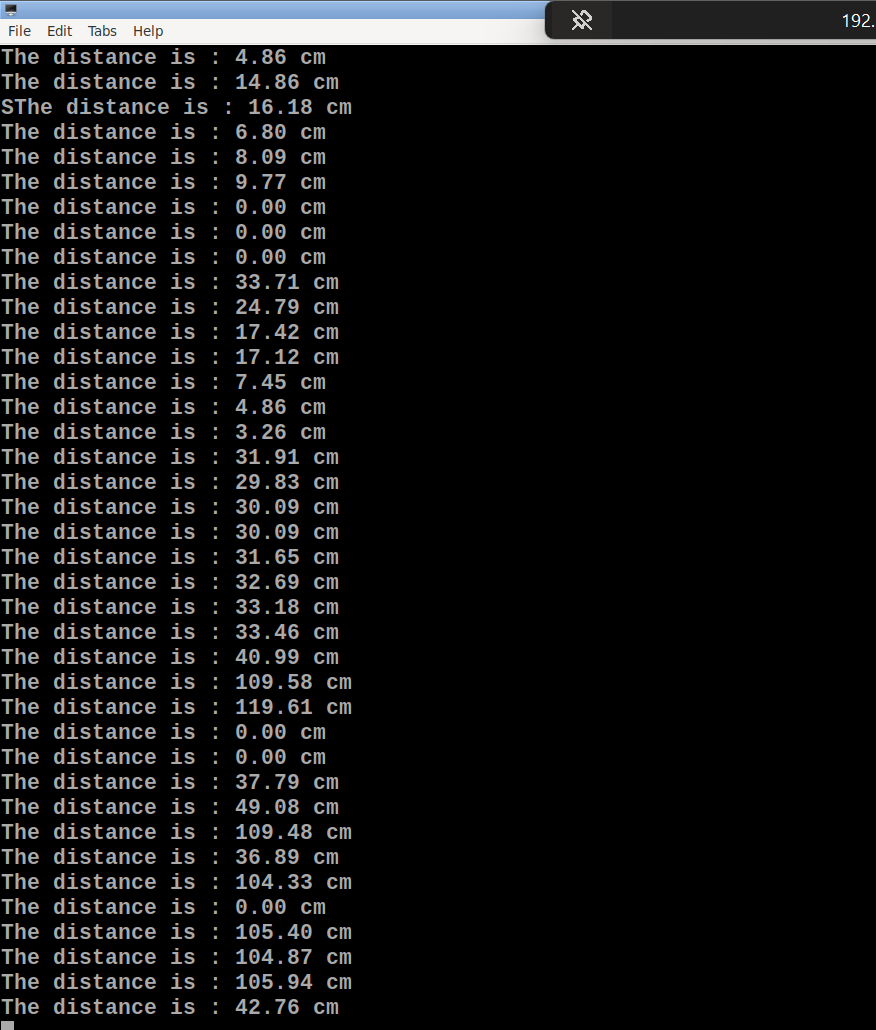
\includegraphics[width=0.5\textwidth]{imagenes/terminal}
	\caption{Foto de la terminal con las medidas del Ultrasónico}
\end{figure}

\begin{figure}[h]
	\centering
	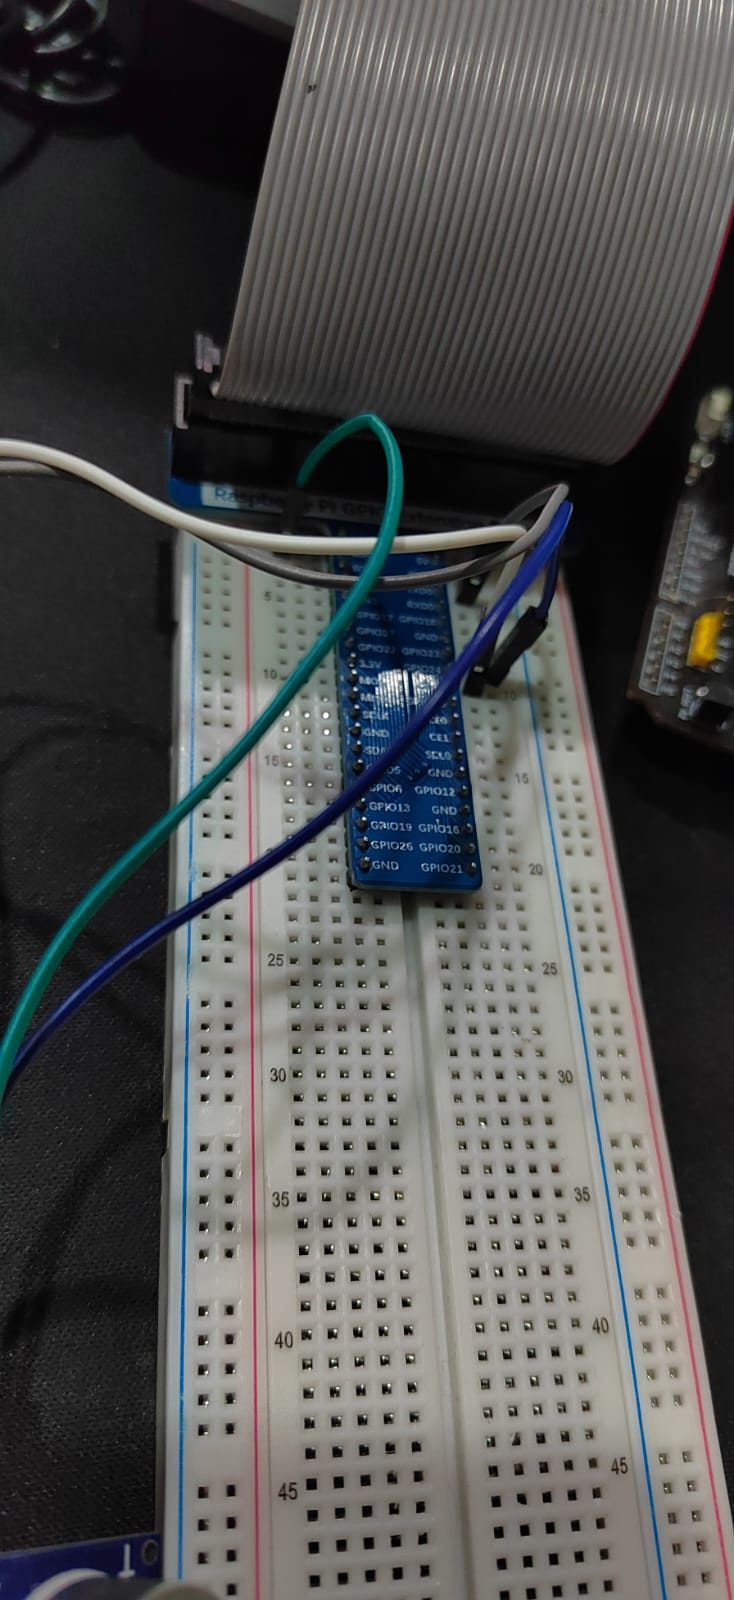
\includegraphics[width=0.5\textwidth]{imagenes/foto1}
	\caption{Foto de las conexiones}
\end{figure}

\begin{figure}[h]
	\centering
	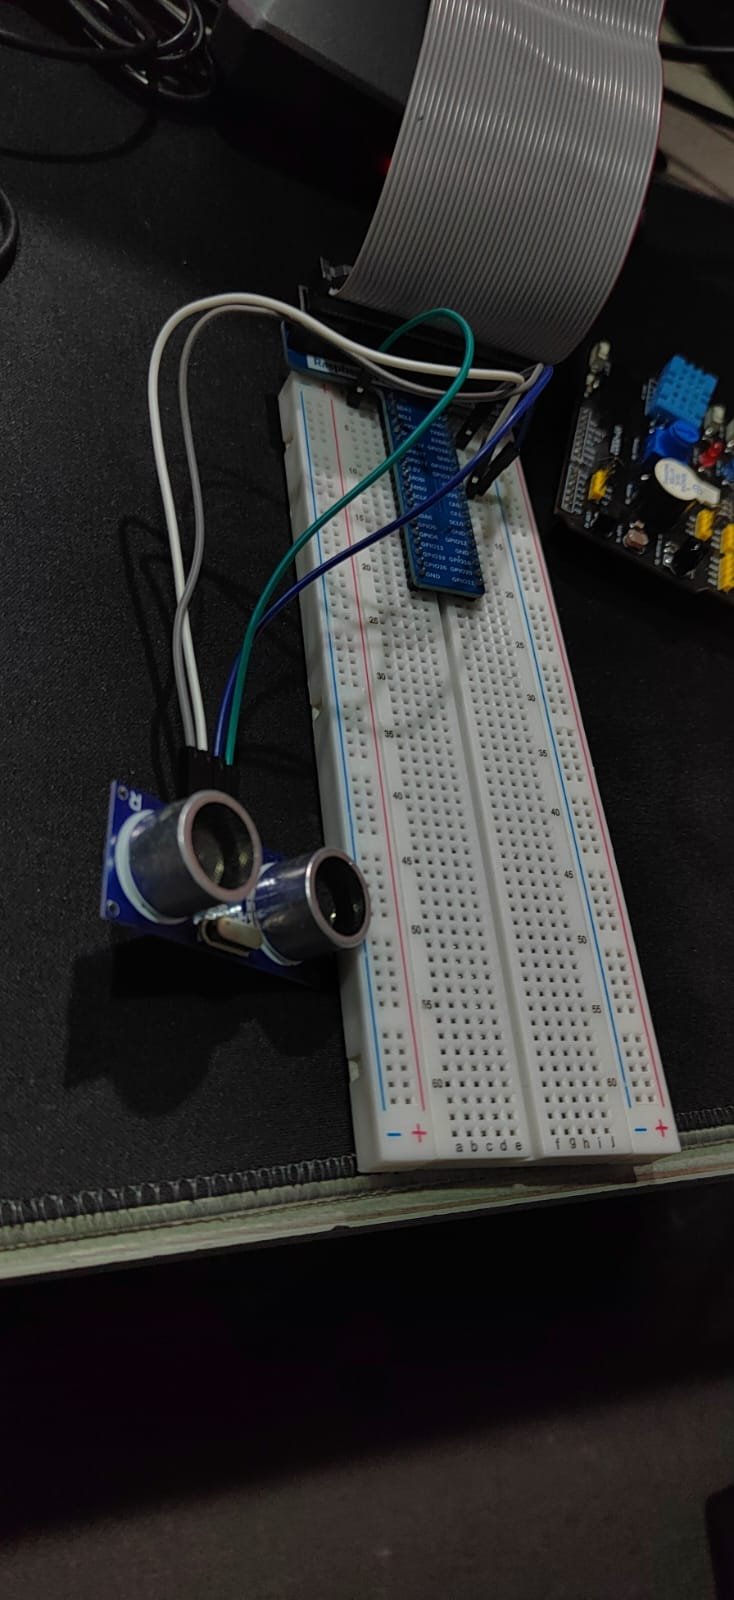
\includegraphics[width=0.5\textwidth]{imagenes/foto2}
	\caption{Divisor de Voltaje}
\end{figure}

\begin{figure}[h]
	\centering
	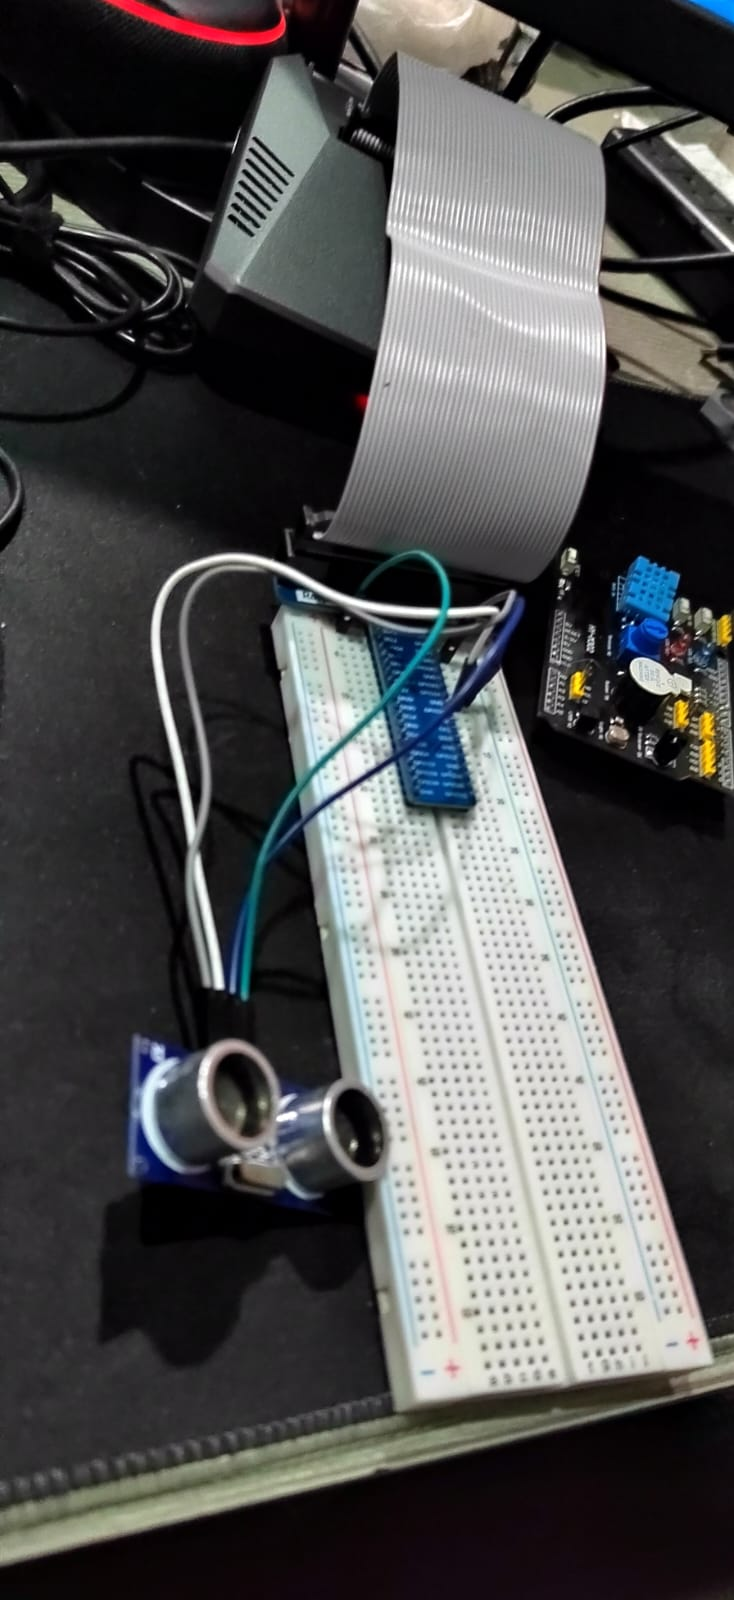
\includegraphics[width=0.5\textwidth]{imagenes/foto3}
	\caption{Conexión Completa}
\end{figure}
